\documentclass[ä5paper, 11pt]{article}
\usepackage[utf8]{inputenc}
\usepackage[spanish]{babel}
\usepackage{listings}
\usepackage[x11names]{xcolor}
\usepackage{graphicx}
\usepackage[lmargin=3cm,rmargin=2.5cm,tmargin=2cm,bmargin=2cm]{geometry}
\usepackage{fancyhdr}
\usepackage{multicol}
\usepackage[export]{adjustbox}
\usepackage{dirtytalk}
\pagestyle{fancy}
\fancyhf{}
\rhead{\thepage}
\lhead{\lefttmark}
\lfoot{Abraham Nava Villavicencio}




%---------------------------------------
\definecolor{rojo}{RGB}{189,004,004}
\pagecolor{rojo}
\definecolor{gris}{RGB}{130,130,130}
\definecolor{azul}{RGB}{013,198,235}
\definecolor{naranja}{RGB}{254,139,032}
\definecolor{verde}{RGB}{128,247,034}
%---------------------------------------
\begin{document}
\begin{center}

\huge{\textbf{Rush Pasión y Gloria}}\\
\Large{Computación - 8180\\
22 de Septiembre de 2022}
\end{center}

\section*{Reseña}
\textcolor{gris}{La pelicula Rush inicia con un discurso de presentación de lo que hace un piloto de formula uno, los riesgos que en ese tiempo corrias al ser piloto de la máxima categoria de automovilismo, así como las posibles razones del porque alguen querria participar en un deporte tan riesgozo, los protagonistas Niki Lauda y James Hunt se conocen desde la formula tres donde empieza su rivalidad, a lo largo de la pelicula nos muestran de forma breve el como llegan a la formula uno y el como avanza su vida personal, el tema central en la pelicula es la temporada del 1976 donde el que se coronaria campeon del mundo lo haria con una diferencia de un solo punto, es la historia de una rivalidad que marco un antes y un despues en el deporte contada con suspenso y acción que te invita a seguir el deporte}
\section*{Reparto}

\begin{multicols}{2}
\textbf{\textcolor{white}{Actores}}
\begin{enumerate}

    \item \fcolorbox{black}{gris}{\textcolor{white}{Daniel Brühl}} Niki Lauda era un tricampeon de la formula uno, una persona muy disciplinada y comprometida con el deporte y con el deseo de ganar
    \item \fcolorbox{black}{gris}{\textcolor{white}{Chris Hemsworth}} James Hunt era una persona que vivia apasionadamente, con una voluntad de ganar inquebrantable, 
    \item \fcolorbox{black}{orange}{Olivia Wilde} Susy Miller fue una modelo actriz y bailarina en su juventud
    \item \fcolorbox{black}{orange}{Alexandra Maria Lara}  Marlene Knaus era una socialité popular y también estaba de moda, trabajando como diseñadora y modelo en los 60s
    
\end{enumerate}
\columnbreak
\textbf{\textcolor{white}{Producción}}
\begin{enumerate}
    \item Ron Howard Director
    \item 	Brian Grazer Productor
    \item Ron Howard Productor
    \item Andrew Eaton Productor
    \item Eric Fellner Productor
    \item Brian Oliver Productor
    \item Peter Morgan Productor y Guionista
\end{enumerate}
\end{multicols}


Niki y James peleando por la posicion en el gran premio de Alemania. 1976

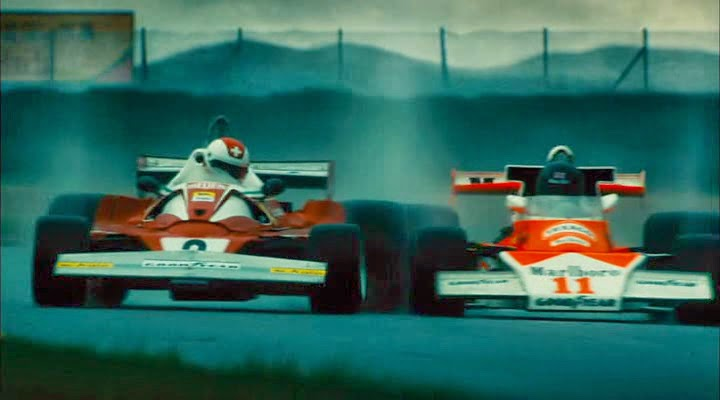
\includegraphics[scale=0.25,angle=15, right]{Imagenes/Alemania 1976.jpg}
   

\newpage
\section*{¿Qué tiene de especial Rush?}

\textcolor{azul}{
Aún para la gente que no es fanática del automovilismo, es sencillo relacionarte con ese deseo de ganar y mostrarle al mundo lo que vales, y esa presisamente es la razón por la que escogí esta película; además la competitividad nos la enseñan desde la escuela y caundo logras encontar una pelicula cuya trama es el poner a dos personajes a competir por ver quien está mas dispuesto a darlo todo para demostrar que es el mejor, esa película siempre será parte de tí}\\

\textcolor{naranja}{Otra de las razones del porque escogí esta pelicula es porque siempre me ha gustado el automovilismo, y a partir de que ví esta pelicula me atrajo aún mas la fromula uno, pues no cualquiera tiene lo que se necesita para poder competir en ella, a parte de una gran cantidad de dinero que te respalde; pues la formula uno es la mas costosa que existe y empieza desde la Super licencia que tienes que tener, un piloto debe estar en una buena forma fisica, pues las fuerzas G que tienen que tolerar con cada frenada o aceleración les puede hacer perder hasta 4 kilogramos de peso en cada carrera, de igual manera la habilidad para controlar un vehiculo de 700 caballos de fuerza tampoco es sencilla de adquirir, si bien en este deporte el auto suele importar casi tanto como el piloto hay casos excepcionales en que un piloto fenomenal gana aún cuando esta en desventaja, y eso es que lo más importa es tu voluntad de ganar}

\textcolor{verde}{La última razón porque solo pidieron tres xd\\ Es que es una pelicula que no te pierde aunque a veces salte en los periodos de tiempo, no se siente tediosa ni te aburre auqnue ya sepas lo que va a pasar y la banda sonora es muy buena, es adoc para los sentimientos que puedes tener al ser fanatico de la formula}\\
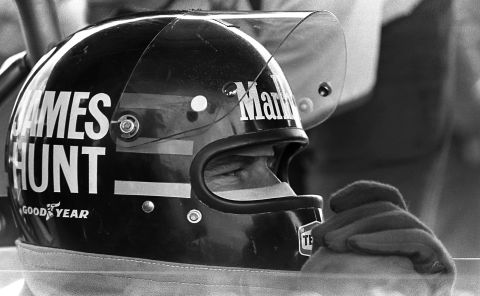
\includegraphics[scale=14, rotate=-18]{Imagenes/james hunt.jpg}{\caption{James hunt, el personaje que le da vida a la pelicula}}

\begin{wrapfigure}
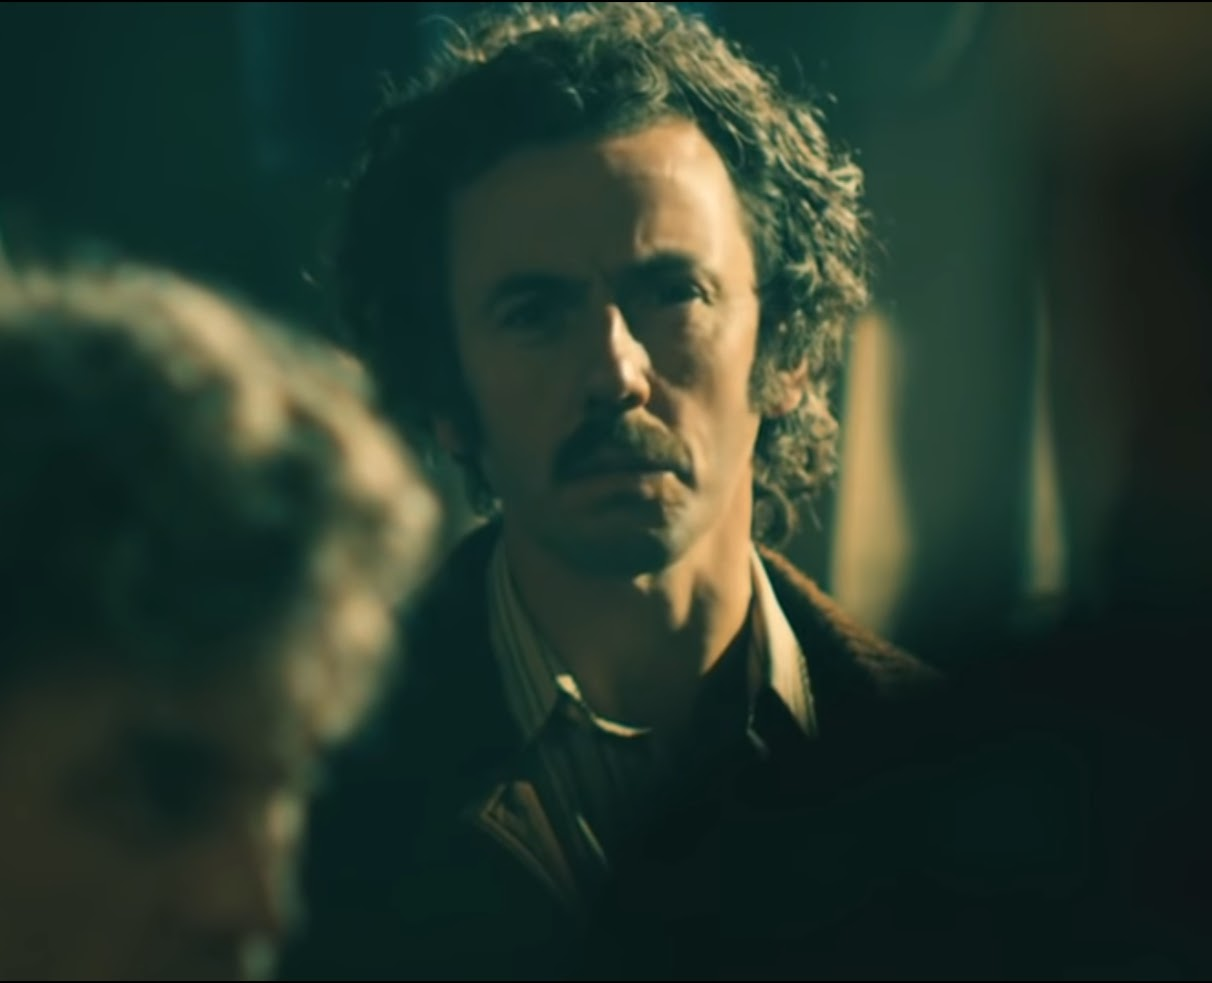
\includegraphics[scale=0.10, rotate=8]{Imagenes/Reportero.jpg} {\caption{El reportero que obtiene su merecido}}
\end{wrapfigure}
\\

\hspace{-2.5cm}\say{{ A wise man gets}

\hspace{-2.5cm}{more from his}

\hspace{-2.5cm}{enemies, than a}

\hspace{-2.5cm}{fool from his friends}}




\end{document}
